% FEATHER — ICDCN 2027 submission (ACM sigconf).
% Restructured full version: Intro (with folded background) -> Literature
% Review -> Methods (Existing Frameworks + Proposed Method, with a limited
% math treatment) -> Experimental Setup -> Results -> Discussion ->
% Feasibility and Constraints -> Conclusion, Limitations & Future Work.
%
% Scope note: this version DOES disclose a limited form of the method
% (the Fisher rank bound as a stated result, one short blindness proof,
% and the streaming algorithm). Full proofs and deep-network results live
% in the complete manuscript in ../../paper/.
%
% Numbers policy: every quantitative claim is taken from our own runs
% (src/experiments/conference_figures.py, src/feather/*, and the verified
% Figure of the synthetic testbed). No unverified latency/ablation numbers.
%
% Compile with pdfLaTeX + BibTeX (Overleaf ships acmart + the bst):
%   main.tex + references.bib + figures/ + acmart.cls + ACM-Reference-Format.bst

\documentclass[sigconf,anonymous]{acmart}

\usepackage{booktabs}
\usepackage{tabularx}
\let\Bbbk\relax
\usepackage{amsmath,amssymb}
\usepackage{algorithm}
\usepackage{algorithmic}
\usepackage{microtype}

\settopmatter{printacmref=true, printccs=true, printfolios=true}

\acmConference[ICDCN 2027]{28th International Conference on Distributed
  Computing and Networking}{January 4--7, 2027}{NITK Surathkal, India}
\acmBooktitle{Proceedings of the 28th International Conference on Distributed
  Computing and Networking (ICDCN 2027)}
\copyrightyear{2027}
\acmYear{2027}
%\acmDOI{}   % assigned at camera-ready
%\acmISBN{}  % assigned at camera-ready

\newcommand{\todo}[1]{\textbf{[TODO: #1]}}

\begin{document}

\title[Toward Label-Free Detection of Harmful Data Drift]{Toward Label-Free
Detection of Harmful Data Drift in Deployed Classifiers}

\author{Anonymous Author(s)}
\affiliation{%
  \institution{Submission under relaxed double-blind review}
  \country{}
}

\begin{abstract}
A deployed classifier's accuracy does not stay fixed. The input stream keeps
moving, and the labels that would tell us the model has started to fail
arrive late or never. Existing label-free monitors split into two camps, and
both have a known weakness. Input-distribution tests raise an alarm on any
change in the inputs, whether or not it costs accuracy. Output-based monitors
read the model's own confidence or entropy, which turn unreliable under
exactly the shifts they are meant to catch. We take a different starting
point. FEATHER (Fisher-Eigenvalue Adaptive Thresholding for Error-Robust
drift detection) watches the geometry of the deployed model itself. It works
in the penultimate feature space and uses the model's Fisher information to
split that space into the directions the model's decisions depend on and the
directions they provably do not. Drift that lands in that second,
output-invisible region is exactly what output monitors miss, and it is what
FEATHER is built to catch. In this paper we give the structural result behind
the method (the empirical Fisher matrix has rank at most $C-1$, so a large
output-invisible subspace always exists), prove that output statistics cannot
see drift inside it, and describe a calibrated streaming monitor that runs as
a cheap, label-free CPU sidecar next to the served model. We validate the
whole chain on a closed-form synthetic stream where every quantity has an
exact answer to check against.
\end{abstract}

\begin{CCSXML}
<ccs2012>
   <concept>
       <concept_id>10010147.10010257.10010258.10010259</concept_id>
       <concept_desc>Computing methodologies~Supervised learning by classification</concept_desc>
       <concept_significance>500</concept_significance>
       </concept>
   <concept>
       <concept_id>10010147.10010257.10010293.10010294</concept_id>
       <concept_desc>Computing methodologies~Neural networks</concept_desc>
       <concept_significance>300</concept_significance>
       </concept>
   <concept>
       <concept_id>10011007.10011074.10011099.10011102.10011103</concept_id>
       <concept_desc>Software and its engineering~Software reliability</concept_desc>
       <concept_significance>300</concept_significance>
       </concept>
 </ccs2012>
\end{CCSXML}

\ccsdesc[500]{Computing methodologies~Supervised learning by classification}
\ccsdesc[300]{Computing methodologies~Neural networks}
\ccsdesc[300]{Software and its engineering~Software reliability}

\keywords{concept drift, model monitoring, dataset shift, label-free
evaluation, machine learning systems}

\maketitle

\section{Introduction}
\label{sec:intro}

Accuracy on launch day is not accuracy forever. Once a model is deployed, the
data it receives starts to change. Users behave differently, a sensor is
replaced, lighting changes, vocabulary shifts, and fraud adapts to the very
detectors built to catch it. Some of these changes barely touch the model.
Others quietly cut its accuracy and leave no trace. Sculley et al.\
\cite{sculley2015debt} named shifting input distributions as one of the main
sources of technical debt in production machine learning, and the problem is
now studied broadly as \emph{concept drift} \cite{gama2014survey,
lu2018learning}.

Let $X \in \mathcal{X}$ be the input and $Y \in \mathcal{Y}$ the label. A
supervised model is trained on samples from a joint distribution $P(X, Y)$.
Any gap between $P(X, Y)$ and the distribution seen in deployment is a
\emph{dataset shift} \cite{quinonero2009dataset}, and it usually gets split
into three kinds. In \emph{covariate shift} the input distribution $P(X)$
changes while $P(Y \mid X)$ stays the same, for example when a camera sensor
is swapped. In \emph{label shift} the class balance $P(Y)$ changes while the
classes themselves stay similar, for example when flu cases rise in season
\cite{lipton2018label}. In \emph{concept shift} $P(Y \mid X)$ itself changes,
for example when a transaction that used to be legitimate is now fraud
\cite{gama2014survey, lu2018learning}. In real streams these kinds arrive
together and at different speeds: abrupt, gradual, incremental, or recurring.
Figure~\ref{fig:drift-types} shows the four speed profiles. A detector tuned
for one of them can miss another.

\begin{figure}[tbp]
\centering
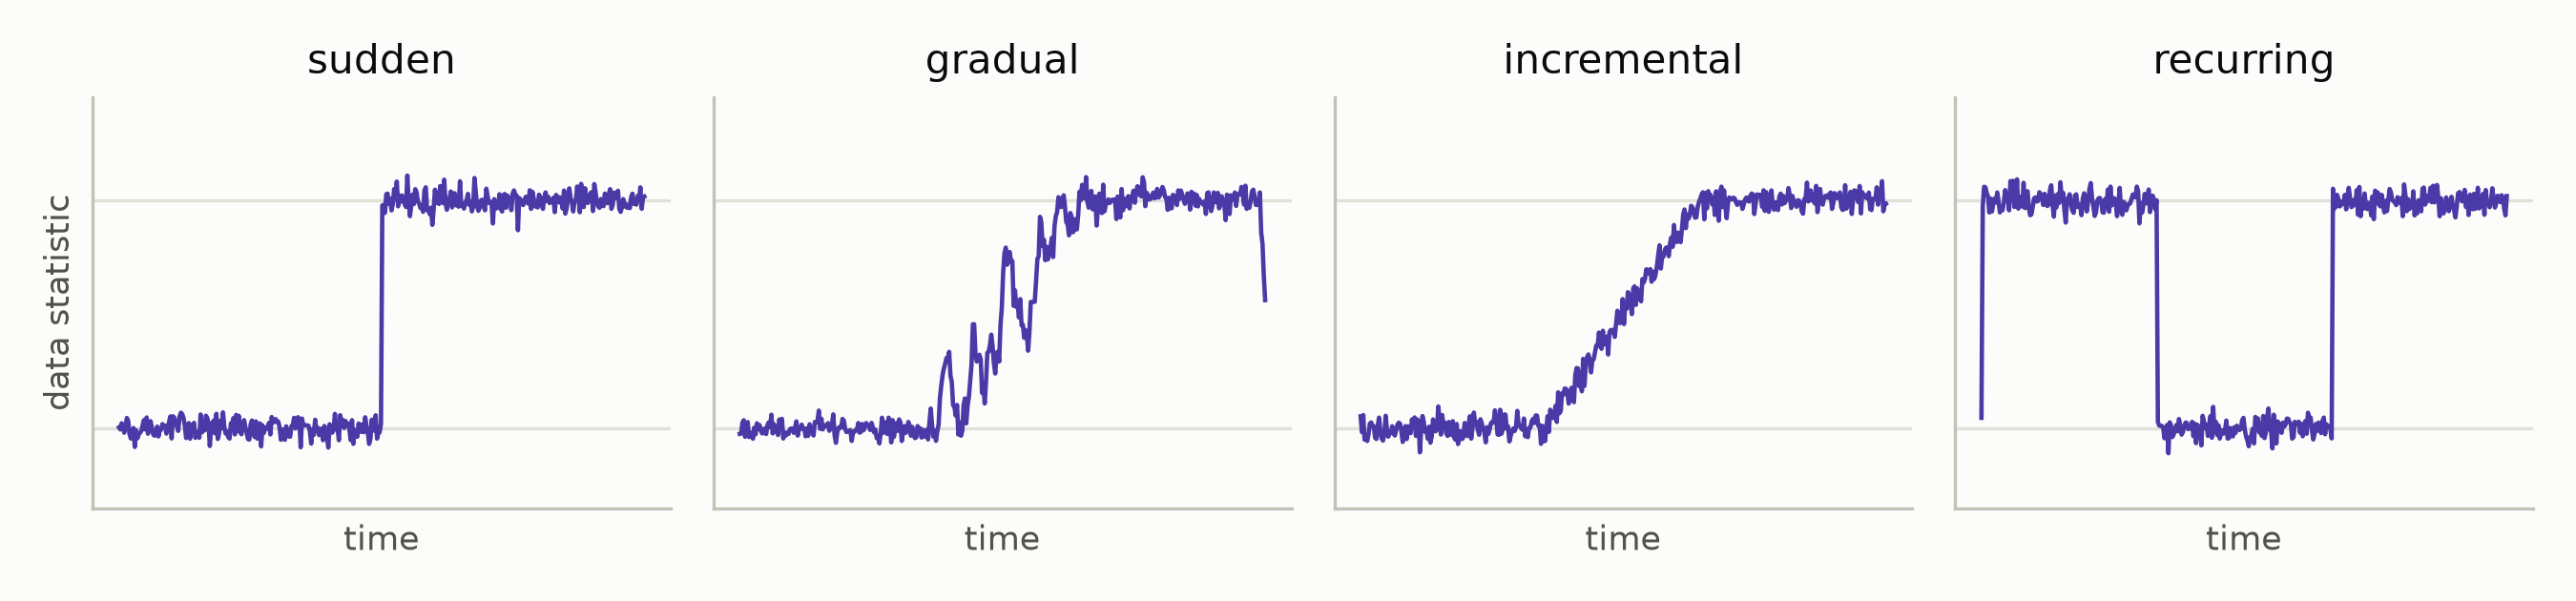
\includegraphics[width=\columnwidth]{figures/drift_types}
\Description{Four line plots of a data statistic against time, labeled
sudden, gradual, incremental, and recurring. In the sudden panel the
statistic steps up once and stays there. In gradual it drifts upward over a
stretch of time. In incremental it rises in stages to a new level. In
recurring it switches back and forth between two levels.}
\caption{The four speeds at which drift arrives in a stream. A monitored
statistic can step up all at once (sudden), climb over a stretch (gradual),
rise in stages (incremental), or come and go (recurring). A monitor tuned for
one profile can easily miss another.}
\label{fig:drift-types}
\end{figure}

These categories say what \emph{kind} of change happened. They do not say
whether the change hurts the model, which is the question an operator
actually has. A large covariate shift may leave a robust model untouched,
while a small shift near a sensitive part of the decision boundary can cost a
lot of accuracy. Following Amoukou et al.\ \cite{amoukou2024sequential}, we
call a shift \emph{harmful} when it causes a measurable drop in the deployed
model's accuracy, and \emph{benign} when it does not. This harmful-versus-benign
split, not the covariate/label/concept split, is what our work is about.
There is good reason for the choice: Rabanser et al.\ \cite{rabanser2019failing}
found that how loudly a shift is detected has little to do with how much
damage it does. A monitor that reports ``something changed'' and stops there
has handed the real work to whoever is on call.

The hard part is not spotting change. Sequential change detectors go back to
Page's CUSUM chart in 1954 \cite{page1954cusum}, and the stream-mining
community has adapted them to learning systems for two decades
\cite{gama2004learning, baena2006eddm, bifet2007adwin, raab2020kswin}. The
hard part is that ``did the data change?'' is the wrong question. In any real
stream the data is always changing. What matters is whether the model still
works, and the labels that would answer that arrive late, in small amounts,
or never. A loan takes months to default; a mis-routed support ticket is
quietly fixed by whoever receives it, with no path back to the model.
Retraining does not rescue this either: it needs those same missing labels,
it does not tell anyone something went wrong, and it does nothing for the
predictions already served \cite{lu2018learning}. Because the labels are
missing, every monitor one can actually deploy is a stand-in for accuracy
rather than a measurement of it, and we argue the field has not looked hard
enough at which stand-in it picks.

This paper introduces FEATHER (Fisher-Eigenvalue Adaptive Thresholding for
Error-Robust drift detection), a monitor built on the geometry of the
deployed model rather than on its raw inputs or its final outputs. FEATHER
works in the penultimate feature space and uses the model's Fisher
information to separate the directions its decisions depend on from the
directions they provably do not. It runs as a lightweight, label-free CPU
sidecar next to the served model. Our contributions are: (i) a structural
result showing the empirical Fisher matrix has rank at most $C-1$, so an
output-invisible subspace of dimension at least $d-C+1$ always exists;
(ii) a short proof that output statistics are blind to drift inside that
subspace; (iii) a calibrated streaming algorithm that watches it under a
chosen false-alarm budget; and (iv) a closed-form synthetic validation of
the whole chain.

\section{Literature Review}
\label{sec:survey}

Work on deployed-model monitoring sorts cleanly into three families by the
signal each one watches: the labels (when available), the inputs, or the
model's own outputs. Table~\ref{tab:families} places them side by side, along
with the geometric family this paper belongs to.

\begin{table*}[t]
\caption{Existing work: deployed-model monitoring families, grouped by the
signal each one watches. The first three are the established families; the
last row is the geometric approach this paper develops.}
\label{tab:families}
\small
\begin{tabularx}{\textwidth}{@{}p{2.9cm} p{4.6cm} c X@{}}
\toprule
Family & Representative methods & Labels online & Monitored signal and main limitation \\
\midrule
Error-rate charts & DDM \cite{gama2004learning}, EDDM \cite{baena2006eddm}, ADWIN \cite{bifet2007adwin} & yes & online classification error; needs the labels the stream does not give \\
Input-distribution tests & MMD \cite{gretton2012kernel}, KSWIN \cite{raab2020kswin}, BBSD \cite{rabanser2019failing} & no & two-sample feature test; performance-agnostic, alarms on benign shift \\
Output-based estimators & MSP \cite{hendrycks2017baseline}, DoC \cite{guillory2021doc}, ATC \cite{garg2022atc}, PUDD \cite{pudd2025}, error proxies \cite{amoukou2024sequential} & no & softmax confidence/entropy; miscalibrated under shift \cite{ovadia2019trust}, blind to null-space drift \\
Geometric (FEATHER, this paper) & FEATHER, score charts \cite{zhang2023score}, ZDP \cite{pandey2025zdp}, activation probes \cite{komorniczak2024parallel} & no & Fisher-weighted feature geometry; label-free, harm-oriented, calibrated \\
\bottomrule
\end{tabularx}
\end{table*}

Error-rate detectors carry statistical process control \cite{page1954cusum}
over to streams. DDM raises an alarm once the online error rate climbs a set
margin above its running minimum \cite{gama2004learning}; EDDM reworks the
idea for gradual drift \cite{baena2006eddm}; ADWIN keeps an adaptive window
and splits it when its two halves disagree, with provable false-positive
bounds \cite{bifet2007adwin}. These ask the right question, but to answer it
they need a label for every prediction, which deployment does not provide.
When labels are late, all this buys is that silent failure becomes
slow-motion failure. The River library \cite{montiel2021river} ships solid
implementations, which at least makes them easy baselines.

Input-distribution tests drop labels and ask instead whether the incoming
inputs still look like the reference data, usually through two-sample
testing. This includes Maximum Mean Discrepancy \cite{gretton2012kernel},
windowed Kolmogorov--Smirnov tests such as KSWIN \cite{raab2020kswin}, and
tests run on the model's representations rather than raw pixels
\cite{rabanser2019failing}; structured cases such as label shift have their
own estimators \cite{lipton2018label}. Their sensitivity is also their
weakness. The test measures how far two distributions are apart, not how much
that distance costs the model. Rabanser et al.\ \cite{rabanser2019failing}
showed these detectors reliably flag synthetic corruptions, including ones
that do no harm, so a monitor that fires on every harmless change soon gets
ignored.

Output-based estimators read the model's own outputs. The
maximum-softmax-probability baseline showed that a classifier's confidence
carries information about whether its prediction is right
\cite{hendrycks2017baseline}. Later methods estimate accuracy from confidence
differences \cite{guillory2021doc}, a learned confidence threshold whose
exceedance rate tracks accuracy \cite{garg2022atc}, or a prediction-uncertainty
index \cite{pudd2025}; the closest to our problem detects harmful shift
sequentially with an error proxy \cite{amoukou2024sequential}, and control
charts have been carried over through score vectors \cite{zhang2023score}.
This family finally asks the operator's question, and often answers it well.
The trouble is the witness. Deep networks are miscalibrated even in
distribution \cite{guo2017calibration}, and get worse under the very shift
the monitor exists to catch \cite{ovadia2019trust}. There is a second, less
discussed problem: a monitor built only on outputs cannot see anything the
outputs do not express. If predictions stay the same after a shift while the
true labels move, an output monitor sees nothing even as accuracy falls. We
show in Section~\ref{sec:methods} that this blind region is not a corner case
but a subspace whose size we can write down exactly.

Geometric methods probe the model's internal representations directly. Out-of-distribution
detection scores samples by class-conditional Mahalanobis distance in feature
space \cite{lee2018mahalanobis}; other lines use score-vector control charts
\cite{zhang2023score}, null-direction probing of language-model
representations \cite{pandey2025zdp}, and label-free activation monitors
\cite{komorniczak2024parallel}. Most of these rank directions by variance or
density rather than by task relevance, so they stay performance-agnostic in
the same way as raw input tests. Benchmarks such as CIFAR-10-C
\cite{hendrycks2019benchmarking} and WILDS \cite{koh2021wilds} test shift
robustness, and systems work \cite{sculley2015debt} stresses that monitoring
must stay light enough not to slow serving.

Three gaps run through all of this. First, input tests treat every feature
direction alike and so alarm on benign covariate shift. Second, output
confidence miscalibrates under shift and is structurally blind to drift that
leaves the outputs unchanged. Third, the existing geometric methods lack
calibrated, low-cost false-alarm control for a zero-label streaming setting.
These gaps frame three questions:

\begin{enumerate}
\item Which feature-space shifts are invisible to any monitor built only on
  the model's output statistics, and can that region be described exactly?
\item Can Fisher-information geometry isolate those output-invisible harmful
  shifts while holding a chosen false-alarm rate?
\item How does such a geometric monitor compare with output estimators, input
  tests, and a task-agnostic covariance baseline?
\end{enumerate}

The rest of the paper is organized as follows. Section~\ref{sec:methods}
develops the existing frameworks and our proposed method, including the
Fisher rank bound, the blindness result, and the streaming algorithm.
Section~\ref{sec:setup} describes the experimental setup and baselines,
Section~\ref{sec:results} reports the synthetic validation,
Section~\ref{sec:outcomes} discusses implications and next steps,
Section~\ref{sec:feasibility} covers feasibility and constraints, and
Section~\ref{sec:conclusion} concludes with limitations.

\section{Methods}
\label{sec:methods}

Table~\ref{tab:notation} lists the notation used in this section.

\begin{table}[htbp]
\caption{Notation used in the FEATHER monitor.}
\label{tab:notation}
\small
\begin{tabularx}{\columnwidth}{@{}l X@{}}
\toprule
Symbol & Meaning \\
\midrule
$X, Y$ & input features and target label \\
$\phi(x)\in\mathbb{R}^d$ & penultimate feature representation \\
$W, b$ & softmax weight matrix ($C\times d$) and bias ($C$) \\
$z(x)$ & logits $z(x)=W\phi(x)+b\in\mathbb{R}^C$ \\
$p(x)$ & softmax output, $p_c = e^{z_c}/\sum_k e^{z_k}$ \\
$g_i$ & score vector $g_i = W^{\top}(e_{y_i}-p(x_i))\in\mathbb{R}^d$ \\
$\mathbf{F}$ & empirical Fisher matrix $\tfrac{1}{n}\sum_i g_i g_i^{\top}\in\mathbb{R}^{d\times d}$ \\
$V_{\text{blind}}$ & basis of $\ker(\mathbf{F})\subset\mathbb{R}^d$ (the blind subspace) \\
$s, m, v$ & per-batch direction, magnitude, and energy statistics \\
$\tau_m, \tau_v$ & bootstrap-calibrated 99th-percentile thresholds \\
\bottomrule
\end{tabularx}
\end{table}

\subsection{Existing Frameworks}
\label{sec:existing}

Label-free monitors work on batches of streaming data $\mathcal{B}_t =
\{x_j\}_{j=1}^b$. Input-based tests compute a distance $d(P_{\text{ref}},
P_{\mathcal{B}_t})$ between the batch and a reference set and alarm when it
crosses a threshold. Because that distance weights every feature direction
the same, it cannot tell a benign shift along the decision boundary from a
harmful shift across it.

Output-based monitors instead track a statistic of the softmax outputs, such
as the mean confidence $\bar c_t = \tfrac{1}{b}\sum_j \max_c p_c(x_j)$ or the
mean entropy, and alarm when it drifts from its reference value. Here a
structural blind spot appears. The outputs come from the logits $z(x) =
W\phi(x)+b$, so any feature-space shift $\Delta\phi$ with $W\Delta\phi = c\,
\mathbf{1}$ (a constant added to every logit) leaves the softmax output
completely unchanged. Such shifts are invisible to \emph{any} output-based
monitor, no matter how it processes the outputs. The next section shows this
invisible set is a subspace whose dimension we can bound exactly.

\subsection{Proposed Method}
\label{sec:proposed}

\paragraph{Fisher geometry and the blind subspace.}
A trained classifier does not use its feature space evenly: some directions
carry the information its decisions turn on, and others carry none. We read
that split off the model's Fisher information, a classical object from
information geometry \cite{amari1998natural}. On a finite reference set
$\{(x_i,y_i)\}_{i=1}^n$ we use the empirical, label-conditioned form
\begin{equation}
\mathbf{F} = \frac{1}{n}\sum_{i=1}^{n} g_i g_i^{\top}, \qquad
g_i = W^{\top}\bigl(e_{y_i}-p(x_i)\bigr),
\end{equation}
which is what a single offline reference set allows one to compute; the gap
to the true Fisher is understood \cite{kunstner2019empirical} and does not
affect the structural property we use. An eigendecomposition $\mathbf{F} = V
\Lambda V^{\top}$ splits $\mathbb{R}^d$ into a task-sensitive subspace
(positive eigenvalues) and a blind subspace $V_{\text{blind}} =
\ker(\mathbf{F})$ (near-zero eigenvalues). FEATHER watches $V_{\text{blind}}$:
drift there is exactly the drift the outputs cannot express, so the monitor
covers the blind spot of the output family while leaving output-visible drift
to the confidence-based tools that already handle it.

Figure~\ref{fig:geometry-toy} shows the idea on a two-class problem. Move the
data across the boundary (red) and predictions, confidence, and entropy all
react; output monitors see it. Move it the same distance along the boundary
(violet) and every output statistic is frozen, even though the data has moved.
Both directions come from the model itself, not from hand-tuning.
Figure~\ref{fig:cov-vs-fisher} contrasts this with a covariance view: variance
or density asks whether a shift is \emph{unusual}, while Fisher asks whether
the model's decision \emph{cares}. The two disagree exactly where it matters
--- a common-looking shift that flips decisions, and a rare-looking shift that
changes nothing.

\begin{figure}[tbp]
\centering
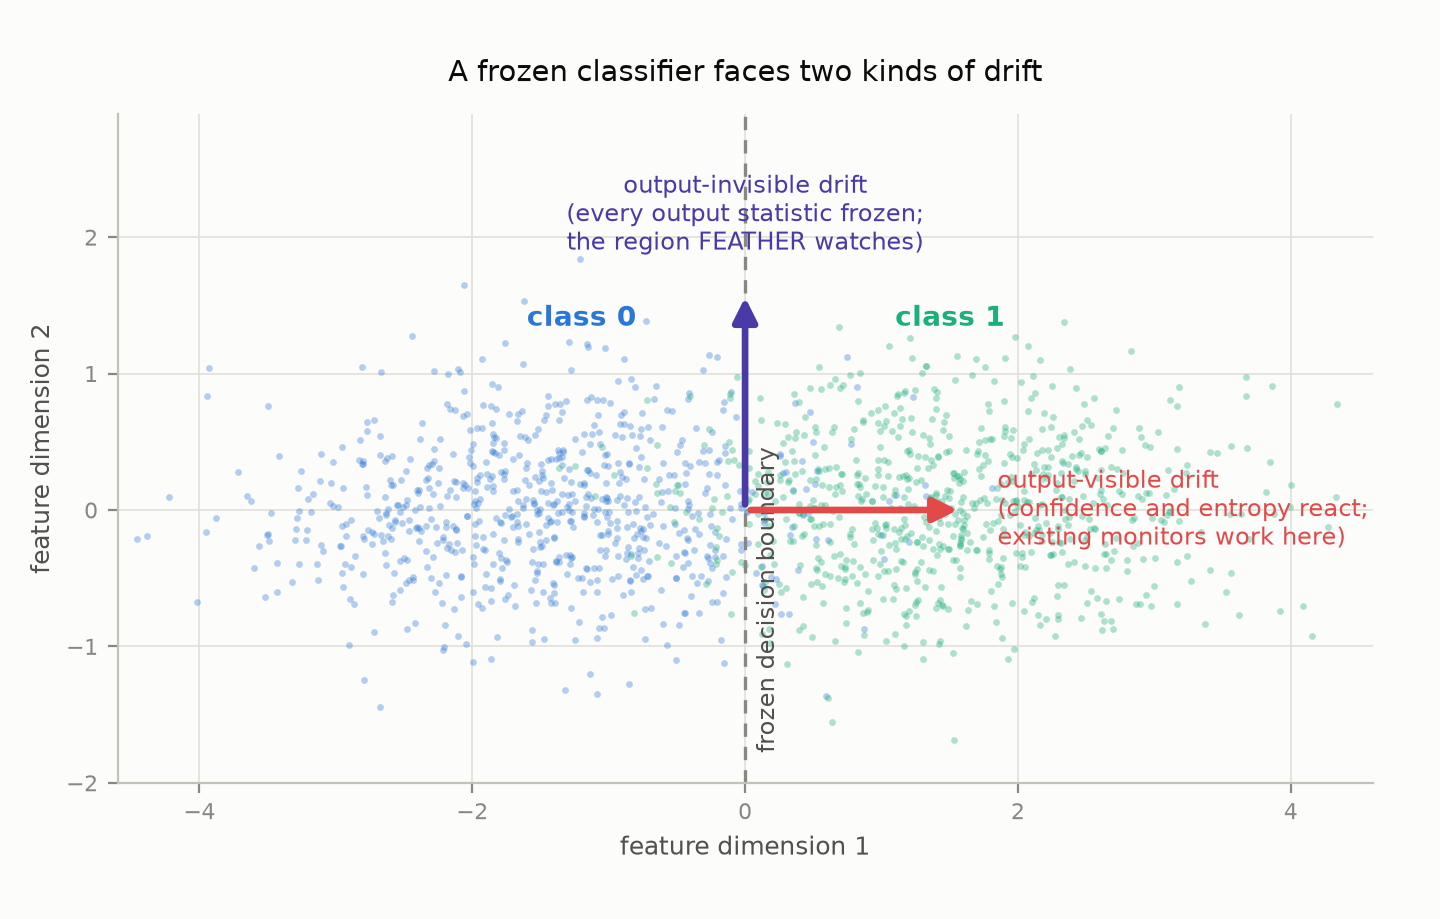
\includegraphics[width=\columnwidth]{figures/geometry_toy}
\Description{Scatter plot of a two-class dataset in two feature dimensions,
split by a dashed vertical decision boundary. A red arrow points across the
boundary, labeled output-visible drift where confidence and entropy react. A
violet arrow points along the boundary, labeled output-invisible drift where
every output statistic is frozen.}
\caption{Two kinds of drift a frozen classifier faces. Across the boundary
(red), the outputs react and existing output monitors work. Along the
boundary (violet), the outputs are frozen while the data moves; this is the
region FEATHER watches. Both directions are read off the model.}
\label{fig:geometry-toy}
\end{figure}

\begin{figure}[tbp]
\centering
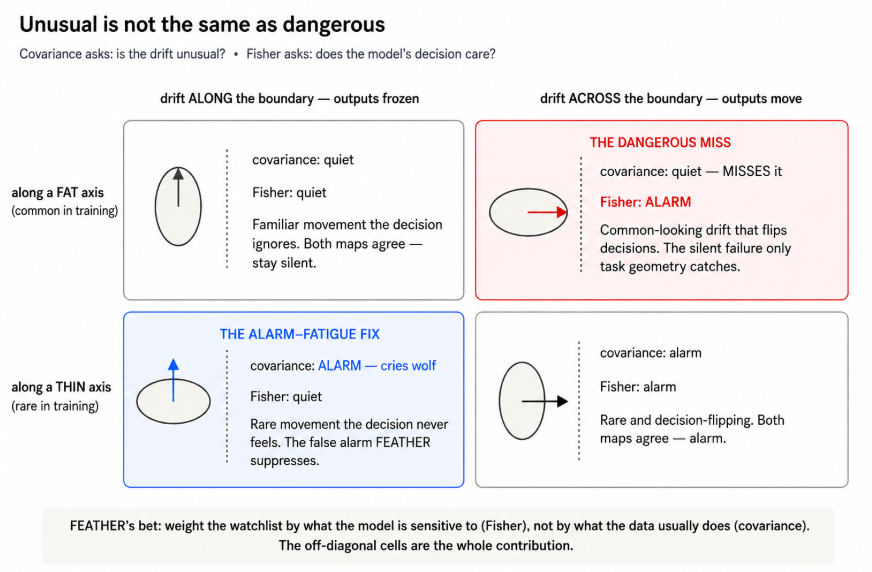
\includegraphics[width=\columnwidth]{figures/Picture1}
\Description{A two-by-two comparison of covariance and Fisher across a fat
axis and a thin axis. Covariance stays quiet on a dangerous boundary-crossing
shift along the fat axis and cries wolf on a harmless shift along the thin
axis, whereas Fisher alarms on the decision-flipping shift and stays quiet on
the harmless one.}
\caption{Unusual is not the same as dangerous. Covariance weights a direction
by how rare the movement is; Fisher weights it by how much the decision
depends on it. They agree on the diagonal and disagree on the two cells that
matter: a common-looking shift that flips decisions (top right) and a
rare-looking shift that changes nothing (bottom left).}
\label{fig:cov-vs-fisher}
\end{figure}

\paragraph{Structural results.}
The blind subspace is not a corner case; its size follows from the softmax
form. Theorem~\ref{thm:rank} states the bound, and
Proposition~\ref{prop:blind} shows output monitors are blind inside it. We
keep the proof of the blindness result, which is the one an operator most
needs to trust, and defer the rank-bound proof and the false-alarm analysis
to the full manuscript.

\begin{theorem}[Fisher rank bound]
\label{thm:rank}
For a $C$-class softmax classifier with penultimate features in
$\mathbb{R}^d$ ($d \ge C$), the empirical Fisher matrix $\mathbf{F}$ over any
reference set satisfies $\operatorname{rank}(\mathbf{F}) \le C-1$, and hence
$\dim(\ker(\mathbf{F})) \ge d-C+1$.
\end{theorem}

The reason is short: each score $g_i = W^{\top}(e_{y_i}-p(x_i))$ is $W^{\top}$
applied to a residual $e_{y_i}-p(x_i)$ that sums to zero, so every $g_i$ lies
in the image of $W^{\top}$ restricted to the $(C-1)$-dimensional zero-sum
hyperplane. The Fisher matrix is an average of outer products of those
vectors, so its rank cannot exceed $C-1$; the null-space bound then follows by
rank--nullity. The practical consequence is that whenever the feature space is
wider than the number of classes, which is the usual case, a large
output-invisible subspace is guaranteed to exist.

\begin{proposition}[Output blindness in $\ker(\mathbf{F})$]
\label{prop:blind}
Let $v \in \ker(\mathbf{F})$, and assume the reference residuals
$\{e_{y_i}-p(x_i)\}$ span the zero-sum hyperplane. Then for any input $x$ and
any scale $\alpha$, the softmax output is unchanged:
$p(\phi(x)+\alpha v) = p(\phi(x))$.
\end{proposition}

\begin{proof}
Since $v \in \ker(\mathbf{F}) = \operatorname{span}\{g_i\}^{\perp}$, we have
$g_i^{\top} v = (e_{y_i}-p(x_i))^{\top} W v = 0$ for every $i$. As the
residuals $\{e_{y_i}-p(x_i)\}$ span the zero-sum hyperplane $\mathcal{S}_C =
\{u : \mathbf{1}^{\top} u = 0\}$, the vector $W v$ is orthogonal to
$\mathcal{S}_C$. In $\mathbb{R}^C$ the orthogonal complement of
$\mathcal{S}_C$ is the line spanned by $\mathbf{1}$, so $W v = c\,\mathbf{1}$
for some scalar $c$. The perturbed logits are then
$z(\phi+\alpha v) = W\phi + b + \alpha c\,\mathbf{1} = z(\phi)+\alpha c\,
\mathbf{1}$, a constant added to every coordinate. The softmax is invariant
to such a constant, so $p(\phi+\alpha v)=p(\phi)$.
\end{proof}

Proposition~\ref{prop:blind} is the formal version of the violet arrow in
Figure~\ref{fig:geometry-toy}: an output monitor cannot react to drift in
$\ker(\mathbf{F})$ at any magnitude, while a monitor that projects onto
$V_{\text{blind}}$ can.

\paragraph{Streaming algorithm.}
FEATHER splits into an offline phase that runs once and an online phase that
runs on every batch, sketched in Figure~\ref{fig:system} and stated in
Algorithm~\ref{alg:feather}. Offline, on a clean reference set, it forms
$\mathbf{F}$, takes the blind basis $V_{\text{blind}}$ by eigendecomposition,
and --- on a \emph{disjoint} calibration split, so no threshold is fit on the
data that shaped the geometry --- computes the reference mean and bootstraps
the 99th-percentile thresholds $\tau_m$ and $\tau_v$ that set the false-alarm
budget. Online, for each unlabeled batch it projects the activations onto
$V_{\text{blind}}$ and computes three statistics: a direction ratio $s$, a
mean-shift magnitude $m$, and an energy $v$ that catches variance or shape
drift the mean misses. It raises a calibrated alarm when $m > \tau_m$ or $v >
\tau_v$. The online step is a single matrix--vector projection per batch, so
it runs on CPU without a GPU or any labels, and adds only a small cost next to
the inference it watches.

\begin{figure*}[t]
\centering
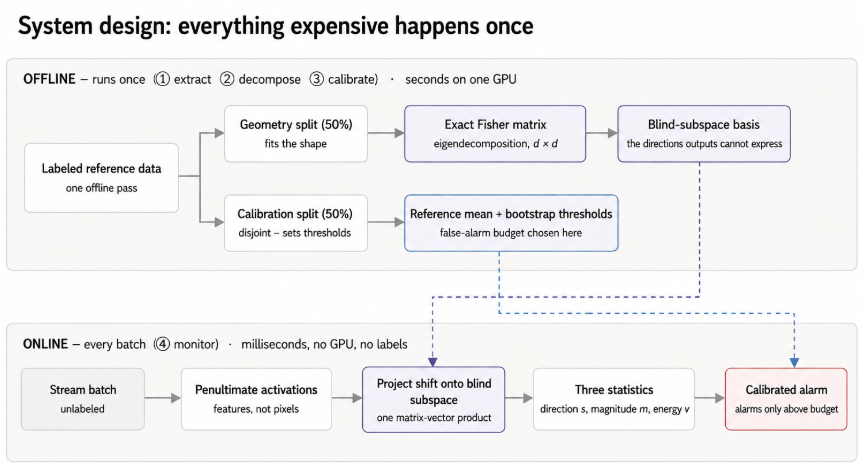
\includegraphics[width=0.92\textwidth]{figures/Picture2}
\Description{A system diagram in two rows. The offline row runs once on a GPU:
labeled reference data is split into a geometry half and a disjoint
calibration half, the exact Fisher matrix is eigendecomposed into a
blind-subspace basis, and the calibration half sets the reference mean and
bootstrap thresholds. The online row runs on CPU for every unlabeled stream
batch: penultimate activations are projected onto the blind subspace with one
matrix-vector product, three statistics are computed, and a calibrated alarm
fires only above the budget.}
\caption{FEATHER as a two-phase system. Everything expensive happens once,
offline on a GPU: fit the Fisher geometry on one half of the reference data
and calibrate thresholds on the disjoint other half. Online, every unlabeled
batch is a single projection onto the blind subspace followed by a calibrated
threshold check, on CPU, with no GPU and no labels.}
\label{fig:system}
\end{figure*}

\begin{algorithm}[htbp]
\caption{FEATHER calibration and streaming monitoring}
\label{alg:feather}
\begin{algorithmic}[1]
\REQUIRE clean reference set $\mathcal{D}_{\text{ref}}$, frozen model $f$,
  false-alarm budget $\alpha$ (we use $\alpha=0.01$)
\ENSURE per-batch alarm $a_t \in \{0,1\}$
\STATE \textbf{Offline (once).} Split $\mathcal{D}_{\text{ref}}$ into disjoint
  geometry and calibration halves.
\STATE Compute scores $g_i = W^{\top}(e_{y_i}-p(x_i))$ and Fisher
  $\mathbf{F} = \tfrac{1}{n}\sum_i g_i g_i^{\top}$ on the geometry half.
\STATE Eigendecompose $\mathbf{F} = V\Lambda V^{\top}$; take the blind basis
  $V_{\text{blind}}$ (near-zero eigenvalues).
\STATE On the calibration half, set the reference mean and bootstrap the
  $(1-\alpha)$-quantile thresholds $\tau_m,\tau_v$.
\STATE \textbf{Online (per batch).}
\FOR{each unlabeled batch $\mathcal{B}_t$}
  \STATE Project activations onto $V_{\text{blind}}$ and compute $s, m, v$.
  \IF{$m > \tau_m$ \textbf{ or } $v > \tau_v$}
    \STATE $a_t \leftarrow 1$ \COMMENT{output-invisible drift flagged}
  \ELSE
    \STATE $a_t \leftarrow 0$
  \ENDIF
\ENDFOR
\end{algorithmic}
\end{algorithm}

The offline phase costs one Fisher build and one eigendecomposition, both
one-time. The online projection is linear in the batch size and the blind
dimension, which is why it fits inside a serving loop as a sidecar rather than
on the request path. We report measured timings in the full manuscript.

\section{Experimental Setup}
\label{sec:setup}

We hold the monitor to four operating criteria. It must be label-free online,
using only unlabeled batches once the one-off offline phase is done. It must
be harm-oriented, so an alarm tracks expected accuracy rather than raw
distribution distance. It must be calibrated, so the operator sets the
steady-state false-alarm rate ahead of time instead of inheriting it from a
hand-tuned constant. And it must be cheap, costing only a small slice of the
inference it watches, or the team will switch it off.

\paragraph{Synthetic testbed.}
Before any deep network, we validate on a stream where every quantity has a
closed-form answer. Two anisotropic Gaussian classes share a covariance, so
the Bayes-optimal boundary is a known line. We use class means $\mu_0 =
(-1.5, 0)$ and $\mu_1 = (1.5, 0)$ and covariance
$\Sigma = \operatorname{diag}(1.0, 0.25)$, which gives boundary normal
$w = (3, 0)$. Drift along the normal $(1,0)$ pushes a class across the
boundary and is output-visible; drift along $(0,1)$ runs parallel to the
boundary and is output-invisible. Streams are 30 batches of 500 samples, with
drift injected at batch 15.

\paragraph{Harm labeling.}
Ground-truth harm is measured, never assumed. Each episode is scored by the
accuracy the deployed model actually loses on held-out labels relative to the
clean episode. In the benchmark protocol an episode is benign below a 2-point
drop and harmful above a 10-point drop; episodes in the gray band between are
dropped from detection scoring rather than forced onto one side.

\paragraph{Benchmarks.}
Beyond the synthetic testbed, the evaluation uses Rotated MNIST, where test
images are rotated by fixed angles to build drift step by step, and CIFAR-10-C
\cite{hendrycks2019benchmarking}, with its 19 corruption types at 5 severities
plus clean data. Models are trained on clean data only, and on several seeds
so we can report run-to-run variation. A natural shift from WILDS
\cite{koh2021wilds}, most likely Camelyon17, is a stretch goal because its
shift is real rather than synthetic. Deep-benchmark numbers are reported in
the full manuscript; here we focus on the synthetic validation.

\paragraph{Baselines.}
We compare against one representative per family in
Table~\ref{tab:families}. Classical error-rate detectors run through River
\cite{montiel2021river} wherever labels are available and act as a
label-having upper bound. Confidence- and entropy-based statistics
\cite{hendrycks2017baseline, garg2022atc} are the label-free output
comparison. The comparison we care about most is against a variance-weighted
covariance monitor that keeps the whole FEATHER pipeline but swaps activation
covariance in where Fisher information goes, at identical calibration. That
one baseline asks a single clean question: does weighting directions by the
task beat weighting them by plain density \cite{lee2018mahalanobis}?

\paragraph{Metrics.}
We report AUROC for separating harmful from benign episodes, but on these
benchmarks it saturates, so we lead with false-alarm behavior on
measured-benign episodes at matched calibration, which keeps telling methods
apart after detection has saturated. We also report post-onset detection delay
and per-batch wall-clock cost against the cost of inference itself.

\section{Results}
\label{sec:results}

On the synthetic testbed the direction our analysis calls output-invisible
matches the analytic null direction to numerical precision, better than
$1-10^{-6}$ in absolute cosine. Figure~\ref{fig:synthetic-demo} runs both
cases from Figure~\ref{fig:geometry-toy}, with drift injected at batch 15.

\begin{figure}[tbp]
\centering
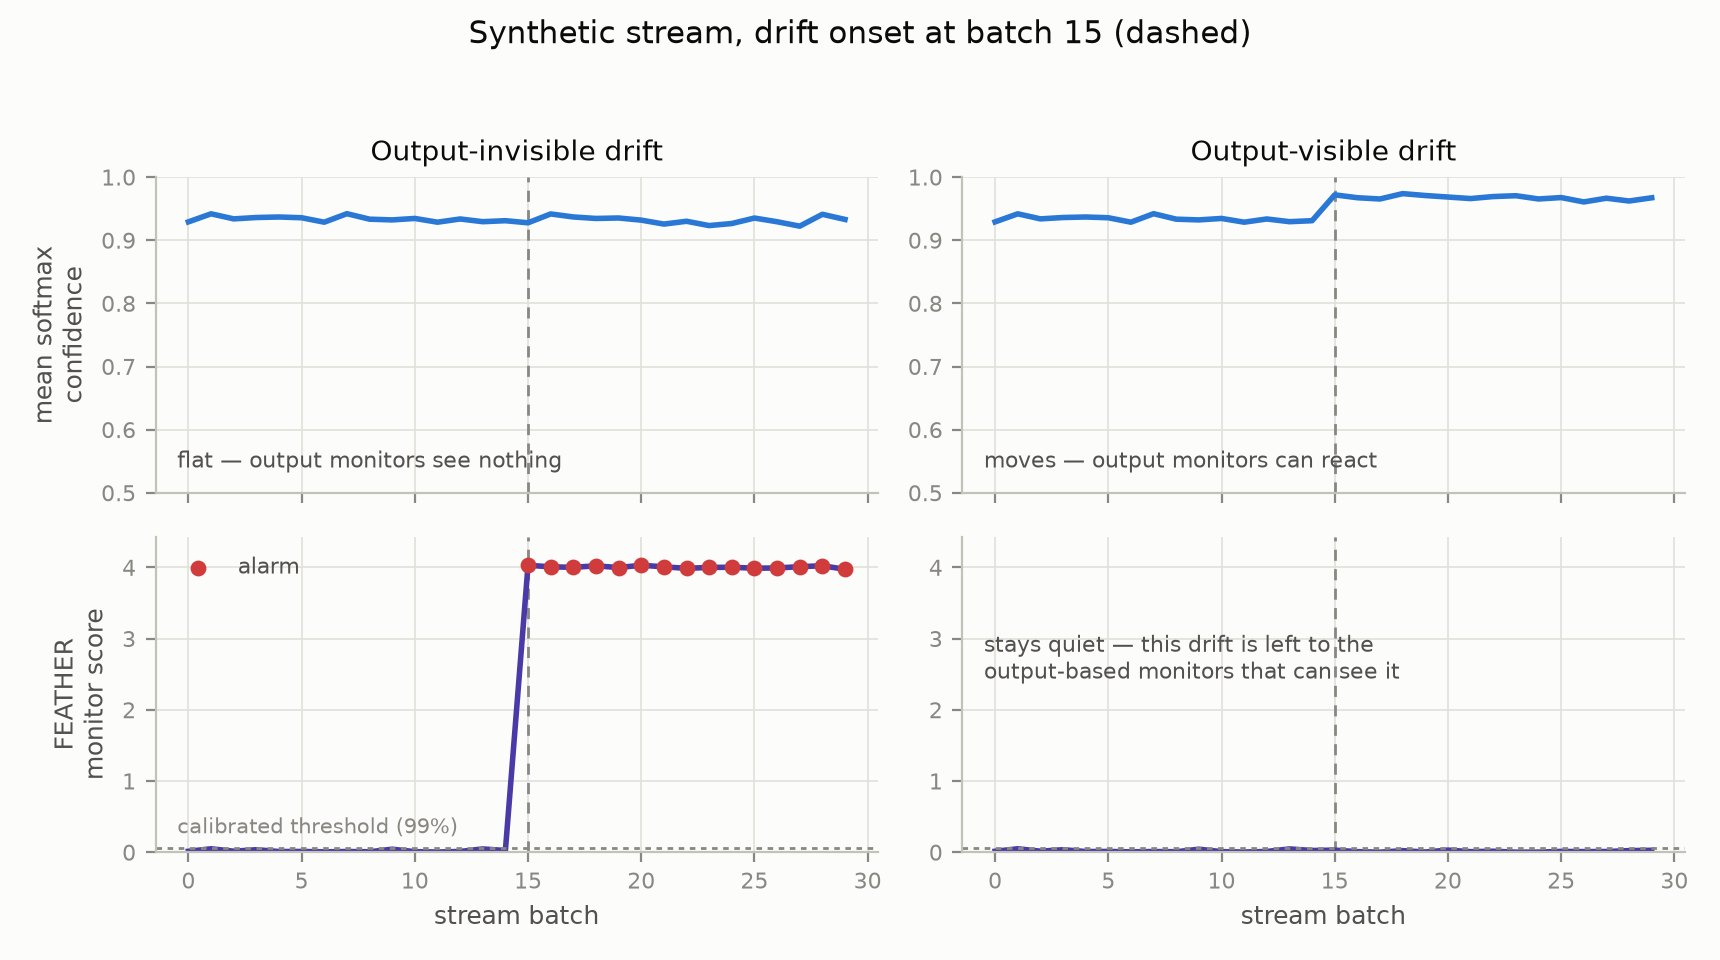
\includegraphics[width=\columnwidth]{figures/synthetic_demo}
\Description{Four panels over a stream of thirty batches with drift onset at
batch fifteen. Under output-invisible drift, mean softmax confidence stays
flat while the FEATHER monitor score jumps above its calibrated threshold and
raises alarms on every post-onset batch. Under output-visible drift,
confidence moves while the monitor score stays at its noise floor with no
alarms.}
\caption{The synthetic testbed in action. Left: output-invisible drift ---
confidence stays flat while FEATHER's score jumps above its calibrated
threshold and flags every post-onset batch. Right: output-visible drift ---
confidence moves (the model becomes confidently wrong, not less confident)
while FEATHER stays quiet and leaves it to the output-based tools that can
see it.}
\label{fig:synthetic-demo}
\end{figure}

Under output-invisible drift (a $4\sigma$ shift along the null direction) the
per-sample change in the model's outputs is below $10^{-10}$, so every
output-based estimator is blind by construction. FEATHER's score jumps from
its noise floor (below $0.05$) to about $4.0$ at batch 15 and stays there,
clearing the calibrated 99th-percentile threshold ($\approx 0.055$) and
flagging all 15 post-onset batches. Under output-visible drift (a $3\sigma$
shift along the boundary normal) the mean softmax confidence moves --- it
\emph{rises} from about $0.93$ to about $0.97$, because the model becomes
confidently wrong rather than uncertain --- so output monitors can react,
while FEATHER stays below its threshold and raises no alarm, avoiding a
redundant second alarm on drift the output family already covers. Across 200
clean batches the false-alarm rate stays within the calibrated budget. The
test suite has 69 unit and integration tests covering the analytic
predictions, the calibration, and the baselines, and runs in a few seconds on
a laptop CPU, so the results here can be re-checked directly.

\section{Discussion}
\label{sec:outcomes}

The synthetic validation makes the central point concrete: a monitor built
only on output statistics has a fixed geometric blind spot, and its size is
set by the softmax rank bound, not by luck. By projecting onto
$\ker(\mathbf{F})$, FEATHER watches exactly that region and defers everything
else to the output family, which avoids the double-alarm behavior that makes
monitors noisy. Because the online step is a single projection evaluated off
the request path, the same design fits a distributed serving setup as a
sidecar: each worker streams its penultimate activations to a monitoring
process that projects and thresholds them, without touching the latency of the
prediction path. We describe this as a deployment design rather than a
measured system; the sidecar has not been benchmarked at cluster scale here.

Two directions look worth pursuing. Extending the blind-subspace idea past the
classifier head to deeper layers needs a way to handle much larger curvature
matrices, where Kronecker-factored approximations \cite{martens2015kfac} keep
the computation manageable, with representational drift in large language
models \cite{pandey2025zdp} as one target. And a benchmark aimed squarely at
the \emph{silent} regime, where realistic drift moves the data without moving
the outputs, similar in spirit to the natural shifts in WILDS
\cite{koh2021wilds}, would test monitors where corruption suites saturate.

\section{Feasibility and Constraints}
\label{sec:feasibility}

The project fits one semester for a team of two. All data is public, so there
is no collection or annotation. The benchmark models train in minutes on a
single 24\,GB GPU, and the monitor itself is cheap enough that the full set of
runs takes hours, not weeks. The stack is PyTorch and torchvision for models
and data, NumPy for the monitor's linear algebra (so the online step runs on
CPU), River \cite{montiel2021river} for the classical baselines, matplotlib
for figures, and pytest for verification. Code, logs, and the scripts that
generate every figure and table are under version control.

Two risks stand out. The theory might not carry from the synthetic setting to
real deep networks; the synthetic gate exists precisely to catch that early,
since every prediction is checked analytically before a deep model is trained,
and we report the outcome either way. And the benchmarks might saturate, with
every detector doing well; if so, the false-alarm metric and the covariance
baseline still separate methods, and the WILDS stretch task adds a setting
that is not synthetic at all.

\section{Conclusion and Limitations}
\label{sec:conclusion}

Label-free monitoring has been stuck between alarming at everything and
trusting a witness that fails under the very shift it should catch. We argued
that what is missing is the geometry of the deployed model, and turned that
into a concrete monitor: a rank bound showing a large output-invisible
subspace always exists, a short proof that output statistics are blind inside
it, and a calibrated streaming algorithm that watches it as a cheap,
label-free sidecar. On a closed-form testbed the monitor catches every
post-onset batch of output-invisible drift while staying within its
false-alarm budget and deferring output-visible drift to the tools that
already see it.

Some limits are worth stating plainly. The rank bound $\operatorname{rank}
(\mathbf{F}) \le C-1$ also caps the blind subspace, so on tasks where the
number of classes approaches the feature dimension the output-invisible region
shrinks. The Fisher we use is the empirical, label-conditioned form, which is
not the true Fisher \cite{kunstner2019empirical}; we argue the gap does not
touch the property we depend on, but the full argument is in the complete
manuscript. Streams with drift in both the sensitive and the blind subspace at
once need multi-component tracking we do not evaluate here. And the strongest
evidence in this paper is synthetic; the deep-network results that would really
test the idea live in the full manuscript, not here.

\bibliographystyle{ACM-Reference-Format}
\bibliography{references}

\end{document}
